\section{Developed Method}
\label{sec:HomographyDevelopedMethod}

Our work aimed to devise a systematic approach to select the ``best'' homography according to the proposed score function. The assumption was that there was no prior knowledge about the quality of individual markers.

Here is the description of the proposed method. Each homography is induced by a single independent marker. The input to our method is multiple sets (i.e., groups) of point correspondences between the warped and the ground-truth (ideal) markers. Therefore, each marker is represented by a unique set of keypoints. The use case of our method is to rank multiple homographies and select the best performing one with respect to the tailor-made score function. Consequently, we require a homography matrix for each marker (a set of point correspondences) on the input. The great advantage comes from the fact that to compute these matrices, any state-of-the-art method can be utilized as a black box. The benefit is that it is capable of ranking the referred homographies without the knowledge of absolute or relative positions of markers in the world (see \figstr{}~\ref{fig:GraphicalAbstract}). However, we have to emphasize that we did not propose any method to simultaneously estimate multiple homographies. We only build upon the existing homography matrices. This particular aspect was the primary source of confusion during the review process of our paper.

Due to our assumption of not knowing the arrangement of markers in the scene, there is no way to create one virtual, compound marker that contains all the keypoints. If we could, then we would employ RANSAC~\cite{fischler1981ransac} or any other sophisticated algorithm to select the best subset of keypoints to estimate the homography. In that scenario, our approach would be useless. We only have information about the relative position of the marker’s keypoints at our disposal, not the markers themselves. As a result, the point correspondence is globally indeterminate. We can only establish a local point correspondence between a single marker and its corresponding ground-truth shape. For the best performance, to obtain the isolated homographies, we suggest the user chooses the most robust method available.

The homography estimation between existing point correspondences is a standard problem on solutions that we heavily rely upon. As already highlighted, we did not contribute to this problem in terms of improving the homography estimation itself. We provided a way to rank the resulting homographies according to the devised score function. We developed a way to,
under certain circumstances, choose the ``best'' homography from multiple existing ones. Therefore, our method could not even be compared to RANSAC, because we tackle a different problem. This suggestion was often brought up during the review process by multiple independent reviewers.

To summarize, there are three following assumptions the proposed method is based upon:
\begin{enumerate}
    \item The markers are geometrically similar, which means that they are allowed to differ only in translation, rotation, and uniform scale in the real world.
    \item The shape of at least one of the used markers is known beforehand.
    \item These markers are positioned on the same planar surface visible in the scene.
\end{enumerate}
One important caveat is that our method handles only transformation from a distorted to the undistorted view of the target plane. Thus, its adoption is restricted solely for the removal of perspective distortion.

We exploited the properties of homography and similarity transformations and expressed them in a single score function, which stands at the core of our contribution. The score function value is exploited as a proxy for homography ranking according to their reprojection error over the entire image using only markers' keypoints. It is only an estimate. The usual use case would be to select the homography with the lowest score, i.e., the highest-ranked matrix, to perform the image rectification with the expectation of obtaining the most accurate reprojection.

\begin{figure}[t]
    \centerline{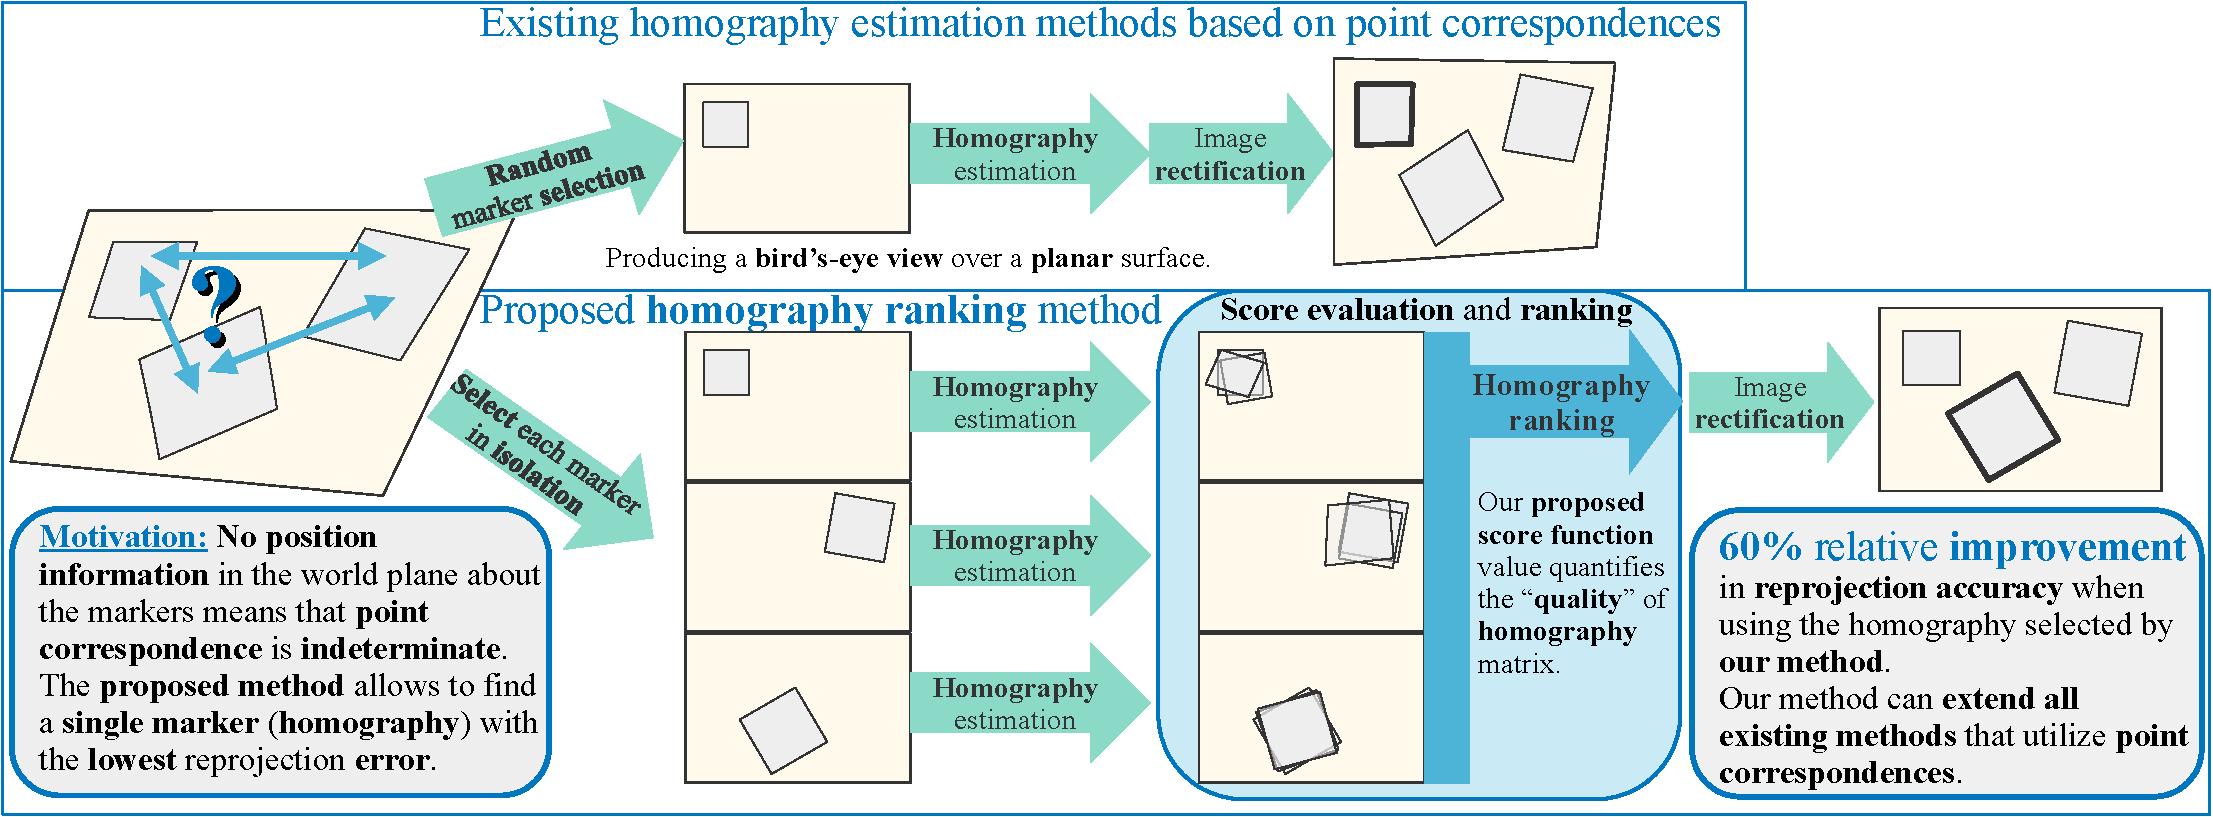
\includegraphics[width=\linewidth]{figures/homography/graphical_abstract.pdf}}
    \caption[Graphical abstract for homography ranking]{Here we present the graphical abstract from our paper. The basic idea is that existing approaches may only estimate an isolated homography for each marker and cannot determine which homography achieves the best reprojection over the entire image. Therefore, we proposed a method to rank isolated homographies obtained from multiple distinct markers to select the best homography. This method extends existing approaches in the post-processing stage, provided that the point correspondences are available and the markers differ only by similarity transformation after rectification. We demonstrated the robustness of our method using a synthetic dataset and showed an approximately $60\%$ relative improvement over the random selection strategy based on the homography estimation from the OpenCV library.}
    \label{fig:GraphicalAbstract}
\end{figure}

\begin{figure}[t]
    \centerline{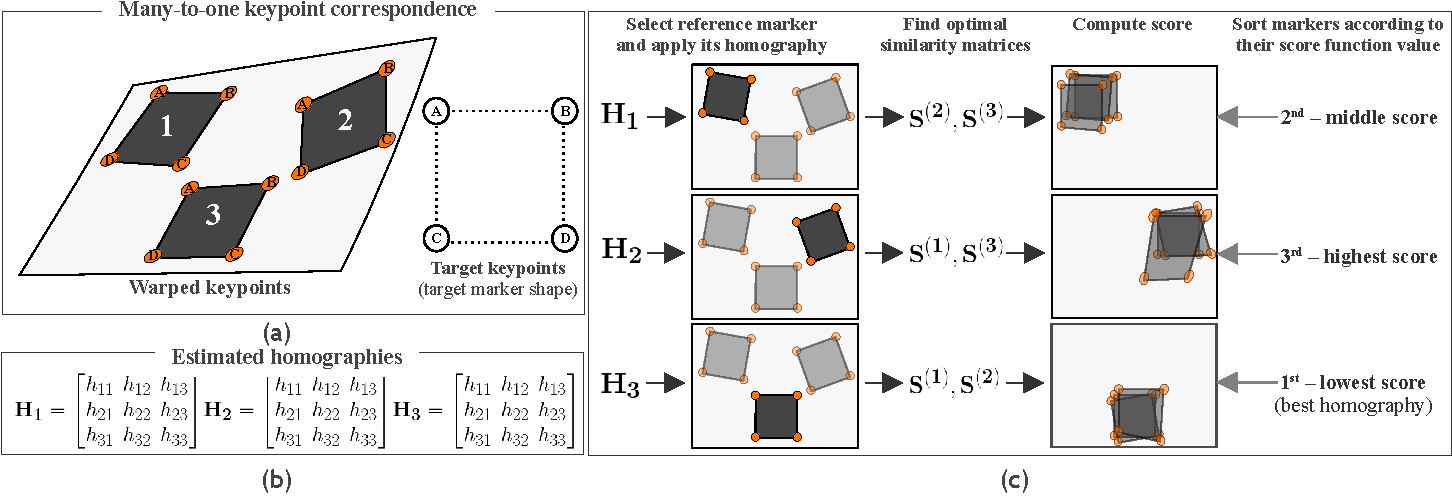
\includegraphics[width=\linewidth]{figures/homography/system_diagram.pdf}}
    \caption[Homography ranking system diagram]{A system diagram depicting the underlying principles behind our method. \imgpartdesc{a} The input consists of a many-to-one point correspondence specified by multiple similar markers together with the information about the ground-truth shape (up to an arbitrary positive scale) of the target marker. \imgpartdesc{b} The assumption is that the isolated homographies related to each marker are ready on the input as well. \imgpartdesc{c} The algorithm processes each marker by applying its corresponding homography matrix to the image to produce a rectified image. Subsequently, it computes optimal similarity matrices using auxiliary markers. These transformations are required for the computation of the score function. The obtained score values then serve for comparison when ranking (sorting in ascending order) the homographies. The homography that ends up ranked first is considered (predicted) to the ``best'' candidate for achieving the minimal reprojection error over the whole image.}
    \label{fig:HomographySystemDiagram}
\end{figure}

A practical advantage of our algorithm is that it is invariant to the underlying homography estimation method. It can, therefore, serve as an extension to all existing or future approaches that handle point correspondences, either as part of run time or a post-processing stage. Moreover, it is computationally very efficient, as it scales well with a quadratic complexity $\func{\Theta}{m^2}$ in the number of markers, which is usually a single-digit number.

Our method utilizes multiple similar markers (see \figstr{}~\ref{fig:HomographySystemDiagram}). The input is point correspondences and homographies estimated for each marker. Each marker becomes the \mbox{reference marker} only once during the course of the algorithm. All the remaining markers serve as \mbox{auxiliary markers}. The reference marker's homography is used to perform the perspective transformation to rectify all the visible markers. To rank which reference markers' homography yields the best reprojection, we exploit auxiliary markers. Auxiliary markers are subsequently mapped onto the target marker using similarity transformations (equation~\ref{eq:SimilarityMatrices}). Then, the transformed keypoints are converted to homogeneous coordinates and the reprojection error is measured as the mean Euclidean distance between the rectified and the target keypoints~\ref{eq:HomographyScoreFunction}. The objective is to minimize the computed quantity. The optimal similarity matrices are just auxiliary and redundant after the algorithm ends.

Let $r$ be the index of the reference marker. The $3 \times 3$ matrices describing similarity transformations are contained in a set $\mset{S} = \cbrackets{\suprbrackets{\mtx{S}}{i} \ |\ i = 1, \dots, m}$, such that
\begin{equation}
    \label{eq:SimilarityMatrices}
    \suprbrackets{\mtx{S}}{i} =
    \begin{cases}
        \begin{aligned}
             & \begin{bmatrix}
                1 & 0 & 0 \\
                0 & 1 & 0 \\
                0 & 0 & 1
            \end{bmatrix} & \text{if } i = r   \\
             & \begin{bmatrix}
                \subsuprbrackets{\mtx{R}}{2 \times 2}{i} & \subsuprbrackets{\mtx{T}}{2 \times 1}{i} \\
                \mathbf{0}_{1 \times 2}                  & 1
            \end{bmatrix} & \text{if }i \neq r \\
        \end{aligned}
    \end{cases},
\end{equation}
for $i = 1, \dots, m$, where
\begin{equation}
    \subsuprbrackets{\mtx{R}}{2 \times 2}{i} =
    \begin{bmatrix}
        \suprbrackets{s}{i} \cdot \func{\cos}{\suprbrackets{\theta}{i}} & -\suprbrackets{s}{i} \cdot \func{\sin}{\suprbrackets{\theta}{i}} \\
        \suprbrackets{s}{i} \cdot \func{\sin}{\suprbrackets{\theta}{i}} & \suprbrackets{s}{i} \cdot \func{\cos}{\suprbrackets{\theta}{i}}
    \end{bmatrix}, \quad
    \subsuprbrackets{\mtx{T}}{2 \times 1}{i} =
    \begin{bmatrix}
        \subsuprbrackets{t}{x}{i} \\
        \subsuprbrackets{t}{y}{i}
    \end{bmatrix}.
\end{equation}
This transformation (besides the identity) involves $4$ \gls{dof}: a single rotation angle $\suprbrackets{\theta}{i}$, two $x$ and $y$ translation coefficients $\subsuprbrackets{t}{x}{i}$, $\subsuprbrackets{t}{y}{i}$, and a scale coefficient $\suprbrackets{s}{i}$. A full affine transformation ($6$ \gls{dof}) would incorporate horizontal and vertical
scales, shear and rotation, and $x$, $y$ offsets~\cite{barath2016novel}. The application of homography that rectifies an image generates a frontal plane that is related to the ground-truth plane by a similarity transformation~\cite{hartley2003multiple, beck2016planar}. Thus, we do not include the shear and we only support uniform scaling. This choice can be easily mathematically justified and can be found in the appendix section of our paper~\cite{ondrasovic2021homography}.

As all the markers share the same planar surface, a valid homography corresponding to any of them by definition to provide a valid perspective projection. However, all perspective projections are subjected to different noise. The endeavor then is to quantify which homography estimation could provide the best perspective projection for the whole plane in the image. To do so, we propose a score function based on the aforementioned constraints. The score function computes a score for individual homographies in along with the estimated similarity matrices corresponding to auxiliary markers as
\begin{equation}
    \label{eq:HomographyScoreFunction}
    \func{\scoref}{\H, \mset{S}} =
    \frac{1}{m}
    \sum_{i = 1}^{m}
    \frobnorm{
        \func{h}{
            \suprbrackets{\mtx{S}}{i}
            \H
            \suprbrackets{\mtx{W}}{i}
        }
        -
        \mtx{T}
    },
\end{equation}
where $\frobnorm{\cdot}$ denotes the Frobenius norm. The function $\func{h}{\cdot}$ converts points to homogeneous coordinates as
\begin{equation}
    \label{eq:HomoCoordsConversion}
    \func{h}{
        \begin{bmatrix}
            x_1 & x_2 & \dots & x_k \\
            y_1 & y_2 & \dots & y_k \\
            z_1 & z_2 & \dots & z_k
        \end{bmatrix}
    } =
    \begin{bmatrix}
        \nicefrac{x_1}{z_1} & \nicefrac{x_2}{z_2} & \dots & \nicefrac{x_k}{z_k} \\
        \nicefrac{y_1}{z_1} & \nicefrac{y_2}{z_2} & \dots & \nicefrac{y_k}{z_k} \\
        1                   & 1                   & \dots & 1
    \end{bmatrix}.
\end{equation}

In what follows, we describe the proposed Algorithm~\ref{alg:HomographyRanking} for homography ranking. Assume a set of warped markers described by the warped keypoints and a single target marker represented by the target keypoints. There is a many-to-one point correspondence linking these objects. Besides, assume that homographies have been estimated for each marker in isolation. Our algorithm ranks the input set of all pairs $\rbrackets{\suprbrackets{\mtx{W}}{i}, \mtx{T}}$, $i = 1, \dots, m$ in ascending order by how well each $i$-th marker preserves the target shape of all the markers in the image after removing the perspective distortion. To measure this objective, the score function defined in equation~\ref{eq:HomographyScoreFunction} comes into place. The algorithm evaluates all markers as candidates for the reference marker. In each iteration, it computes optimal similarity matrices belonging to the auxiliary markers in the rectified plane, i.e., after applying the perspective projection induced by the current homography. The aim is to find a homography with a minimal score. The algorithmic complexity is quadratic in the number of markers, thus $\func{\Theta}{m \rbrackets{m - 1} + m \func{\text{log}_2}{m}} \simeq \func{\Theta}{m^2}$.

\def\hmatrices{\boldsymbol{\bar{H}}}
\def\scoref{\mathcal{F}}

\begin{algorithm}[t]
    \caption{Homography Ranking}
    \label{alg:HomographyRanking}
    \begin{algorithmic}[1]
        \State $\hmatrices \gets \arraydef \left[ m \right]$
        \Comment{output array of homographies}

        \State $\scores \gets \arraydef \left[ m \right]$
        \Comment{array of scores}

        \For{$i \gets 1, \dots , m$}

        \State $\hmatrices \left[ i \right] \gets$
        \Call{homography}{$\suprbrackets{\mtx{W}}{i}$, $\mtx{T}$}
        \Comment{retrieve or estimate perspective}

        \State $\suprbrackets{\mtx{\bar{S}}}{i} \gets \mtx{I}_{3 \times 3}$

        \State $\mset{\bar{S}} \gets \cbrackets{\suprbrackets{\mtx{\bar{S}}}{i}}$
        \Comment{set of similarity matrices}

        \ForAll{$j$ : $\cbrackets{1, \dots, m} - \cbrackets{i}$}

        \State $\suprbrackets{\mtx{\bar{S}}}{j} \gets$ \Call{similarity}{$\hmatrices \left[ i \right] \cdot \suprbrackets{\mtx{W}}{j}$, $\mtx{T }$}

        \State$\mset{\bar{S}} \gets \mset{\bar{S}} \cup \suprbrackets{\mtx{\bar{S}}}{j}$
        \EndFor

        \State $\scores \left[ i \right] \gets \func{\scoref}{\hmatrices \left[ i \right], \mset{\bar{S}}}$
        \Comment{evaluate score function \ref{eq:HomographyScoreFunction}}
        \EndFor
        \State $\sortres \gets \Call{argsort}{\scores}$
        \Comment{indirect sort}

        \State \Return $\hmatrices, \sortres$
    \end{algorithmic}
\end{algorithm}

It is important to remark that the two functions used to compute the homography and similarity matrices in the pseudocode above may stand for arbitrary methods that produce the required transformations.

The score function \ref{eq:HomographyScoreFunction} is just a proxy for the reprojection error computed over the whole image. Since we utilize only a small subset of points from the entire image, which may be subjected to noise, the assumption that the ``best'' homography is the one our method ranks as first may not hold in every case. In very few cases, the marker that achieves the lowest score function value does reconstruct the remaining markers the best, but not the overall image. Nevertheless, the conducted experiments show that our method consistently preserves its performance under various conditions.
